\documentclass{article}
\usepackage[a4paper,margin= 2cm]{geometry}
\usepackage{graphicx}
\usepackage{caption}
\usepackage{subcaption}

\title{\LARGE{\bf{Task 2 Overview}}}
\author{\Large{\bf{Kirtan Patel - AE19B038}}}
\date{}

\begin{document}

\maketitle 

\section{Linear Regression}
Linear regression is an algorithm used to predict, or visualize, a relationship between two different features/variables. In linear regression tasks, there are two kinds of variables being examined: the dependent variable and the independent variable. The independent variable is the variable that stands by itself, not impacted by the other variable. As the independent variable is adjusted, the levels of the dependent variable will fluctuate. The dependent variable is the variable that is being studied, and it is what the regression model solves for/attempts to predict. In linear regression tasks, every observation/instance is comprised of both the dependent variable value and the independent variable value.\\ 

The function of a regression model is to determine a linear function between the X and Y variables that best describes the relationship between the two variables. In linear regression, it’s assumed that Y can be calculated from some combination of the input variables. The relationship between the input variables (X) and the target variables (Y) can be portrayed by drawing a line through the points in the graph. The line represents the function that best describes the relationship between X and Y. The goal is to find an optimal “regression line”, or the line/function that best fits the data.

\section{Task 2}
In this Task, we are given 3 datasets, each consisting of 200 data points. We wrote an Octave code to perform Linear Regression on each dataset, taking the first 50,100 and 200 datapoints one after the other.

Plotting the Regression line as 
\[Y = mX + c\]
we record the values obtained for m and c. Based on the behaviour of m and c, we infer the type of data given.\\ 

We even have to suggest a model that would work better (instead of Y = mX + c) and justify our suggestion.

\section{Recorded Results}

After calculating the Regression Line Variables using Gaussian Elimination to invert matrix A, we get the following values of slop (m) and intercept (c) for the Regression Line Equation \[ Y = mX + c\]
\begin{table}
	\begin{minipage}[b]{.30\textwidth}
		\centering
		\begin{tabular}{| l || l | l |}
			\hline
			Data-1 & m & c \\
			\hline \hline
			50 points & 2.0113 & 1.1880\\
			\hline 
			100 points & 2.0080 & 1.2660\\
			\hline 
			200 points & 2.0057 & 1.3771\\
			\hline
		\end{tabular}
	\end{minipage}\qquad
	\begin{minipage}[b]{.30\textwidth}
		\centering
		\begin{tabular}{| l || l | l |}
			\hline
			Data-2 & m & c \\
			\hline \hline
			50 points & 2.0111 & 1.1956\\
			\hline 
			100 points & 2.0079 & 1.2719\\
			\hline 
			200 points & 2.0056 & 1.3810\\
			\hline
		\end{tabular}
	\end{minipage}\qquad
	\begin{minipage}[b]{.30\textwidth}
		\centering
		\begin{tabular}{| l || l | l |}
			\hline
			Data-3 & m & c \\
			\hline \hline
			50 points & 2.0000 & 1.0053\\
			\hline 
			100 points & 2.0000 & 1.0054\\
			\hline 
			200 points & 2.0000 & 1.0049\\
			\hline
		\end{tabular}
\end{minipage}
	\caption{Tabulated Results of the Regression Line slope and intercept}
	\label{tab:revpol-2}
\end{table}
\pagebreak

\section{Inference}
 Here I have plotted both values, the slope of the Regression line and the intercept of the Regression line, against the Number of Data-points.This is helpful in analyzing the nature of the values in increase in number of data-points.

\begin{figure}[htbp]
	\begin{minipage}[b]{0.5\linewidth}
		\centering
		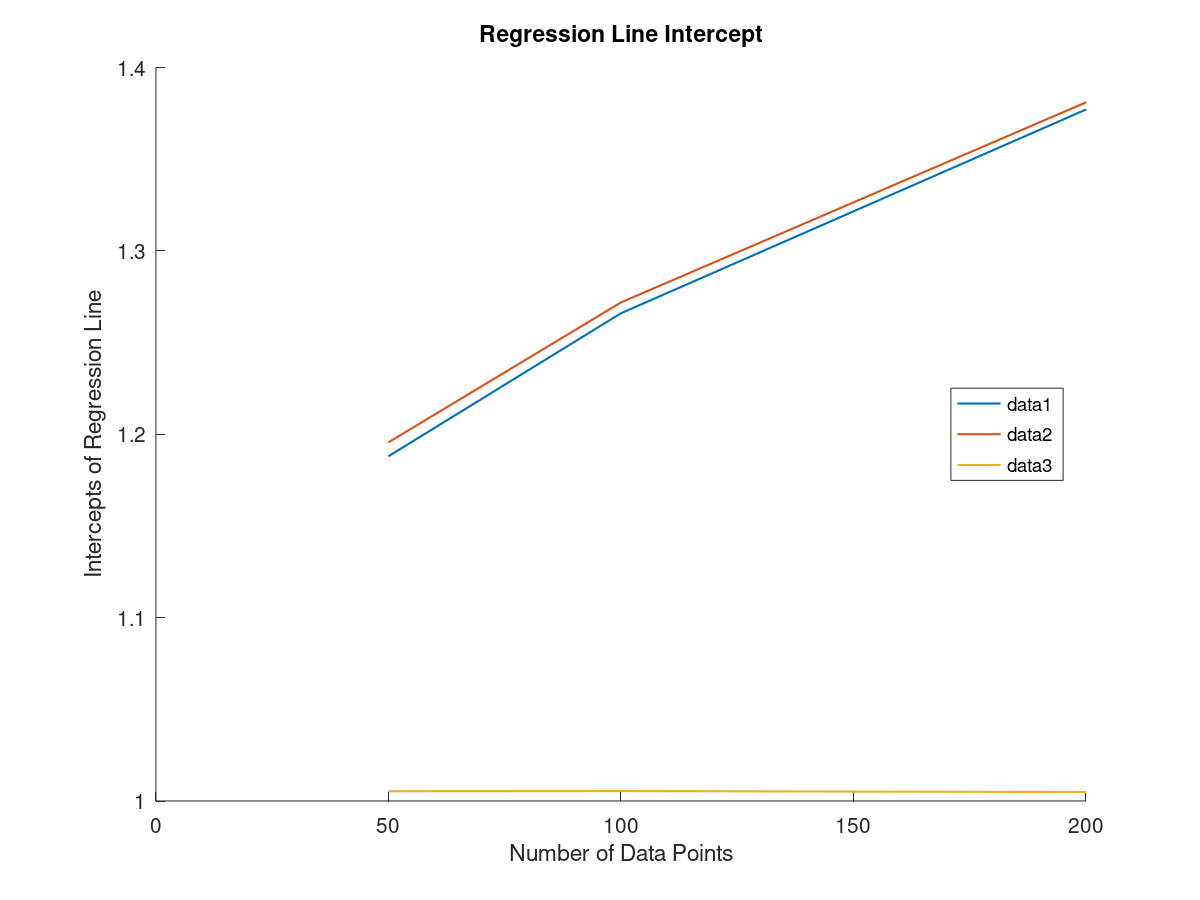
\includegraphics[width=\linewidth]{Regression Line intercept Plot.png}
		\caption{Regression Line intercept Plot}
		\label{fig:chapter001_dist_001}
	\end{minipage}
	\hspace{0.5cm}
	\begin{minipage}[b]{0.5\linewidth}
		\centering
		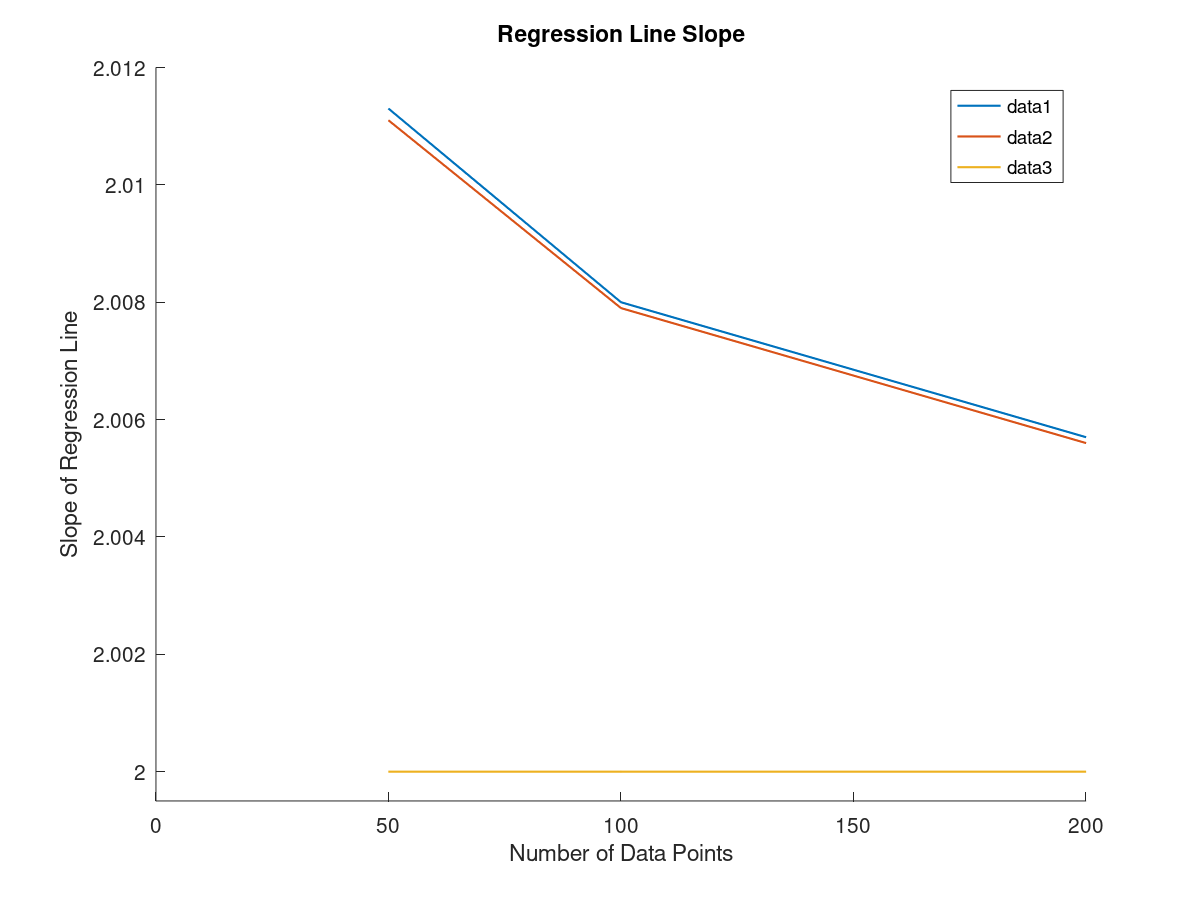
\includegraphics[width=\linewidth]{Regression Line Slope Plot.png}
		\caption{Regression Line Slope Plot}
		\label{fig:chapter001_reward_001}
	\end{minipage}
\end{figure}

For {\bf data1} and {\bf data2} we can see that both the quantities converge to a finite value as we increase the number of data-points. This verifies the fact that the model chosen is correct.\\

If the data had been a better fit for a polynomial of a higher degree, the values of slope and intercept would diverge, as the values would increase more and more rapidly as the number of observations increase.\\

Thus, The linear model is a good fit for the given data. This is shown more clearly by plotting the data and the Regression Line.\\
\\

For {\bf data3}, increase in number of data points gave no change in the slope of the regression line, thus it is possible to infer that data3 is the dataset for which the Linear Regression Model is the best fit.\\

The change in the intercept is also random and not monotonic as we increase the number of data points and hence taking more data points might help in reducing the error.\\
\\

Furthermore we can say that Dataset3 is more linear than Dataset1 and Dataset2.\\
\\

Apart from the nature of regression line for each dataset, we can compare the 3 data sets among themselves as well with the given data of regression line slope and intercept.\\

Dataset 3 has the lowest intercept as well as the lowest slope, and hence it's regression line never crosses that of dataset 1 and 2.\\

Dataset 2 has a higher intercept than Dataset 1 but a lower slope, and hence the regression lines meet at some number of data points (X increases as the number of data points increases). This is significant is before the intersection, Dataset2 gives a higher output value Y for a given X, but after that it is Dataset1 which gives the higher output value.
\pagebreak

\section{Scatter Plot with Regression Line}
\subsection{Dataset 1}
\begin{figure} [!ht]
	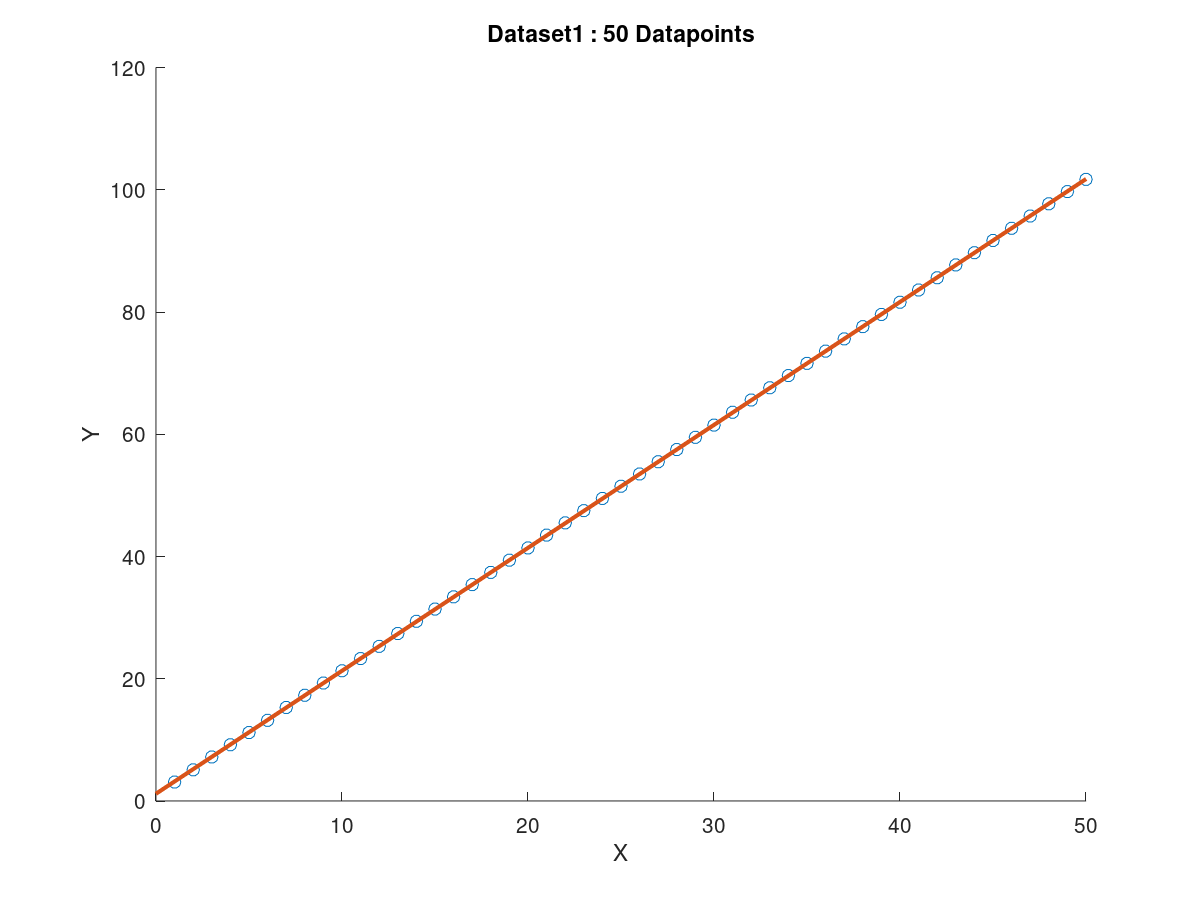
\includegraphics[width=.55\textwidth]{D1-50.png}\hfill
	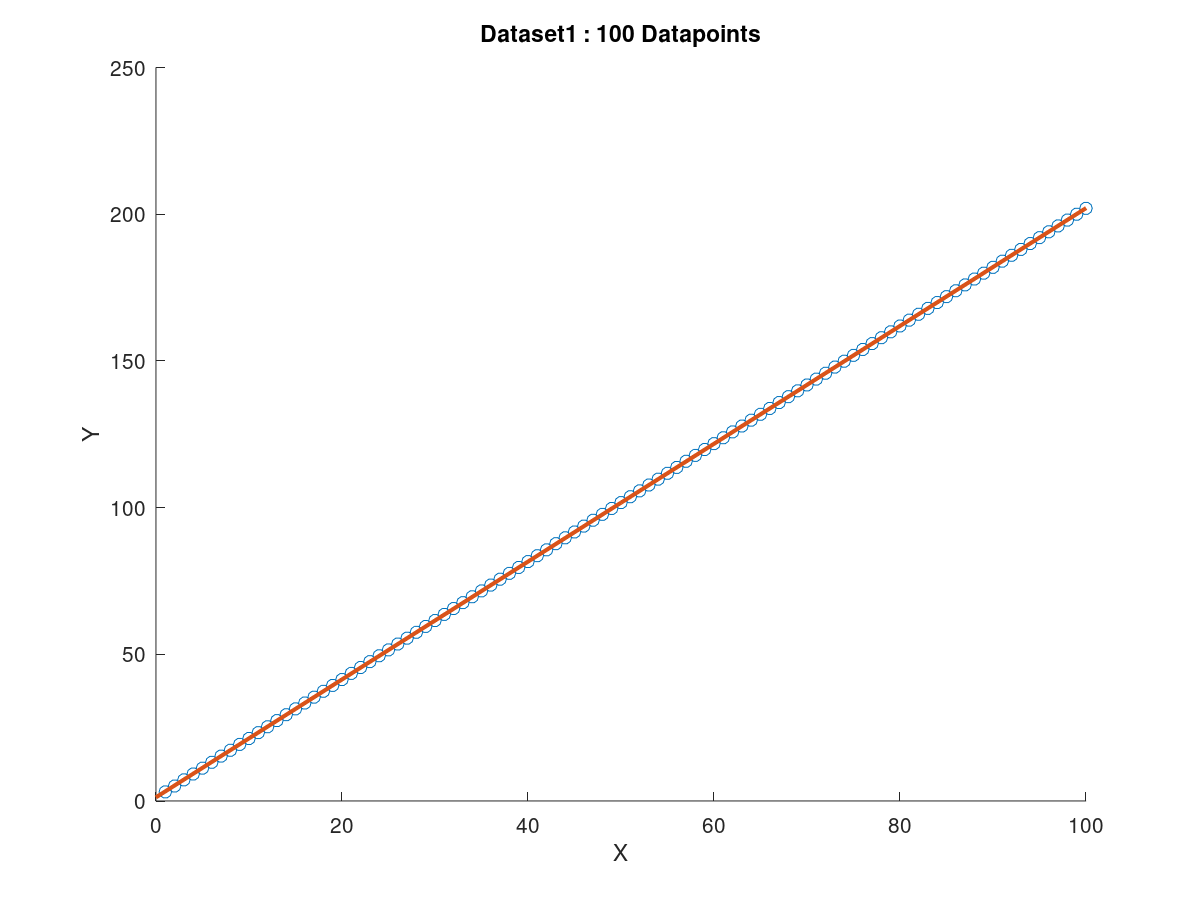
\includegraphics[width=.55\textwidth]{D1-100.png}\hfill
	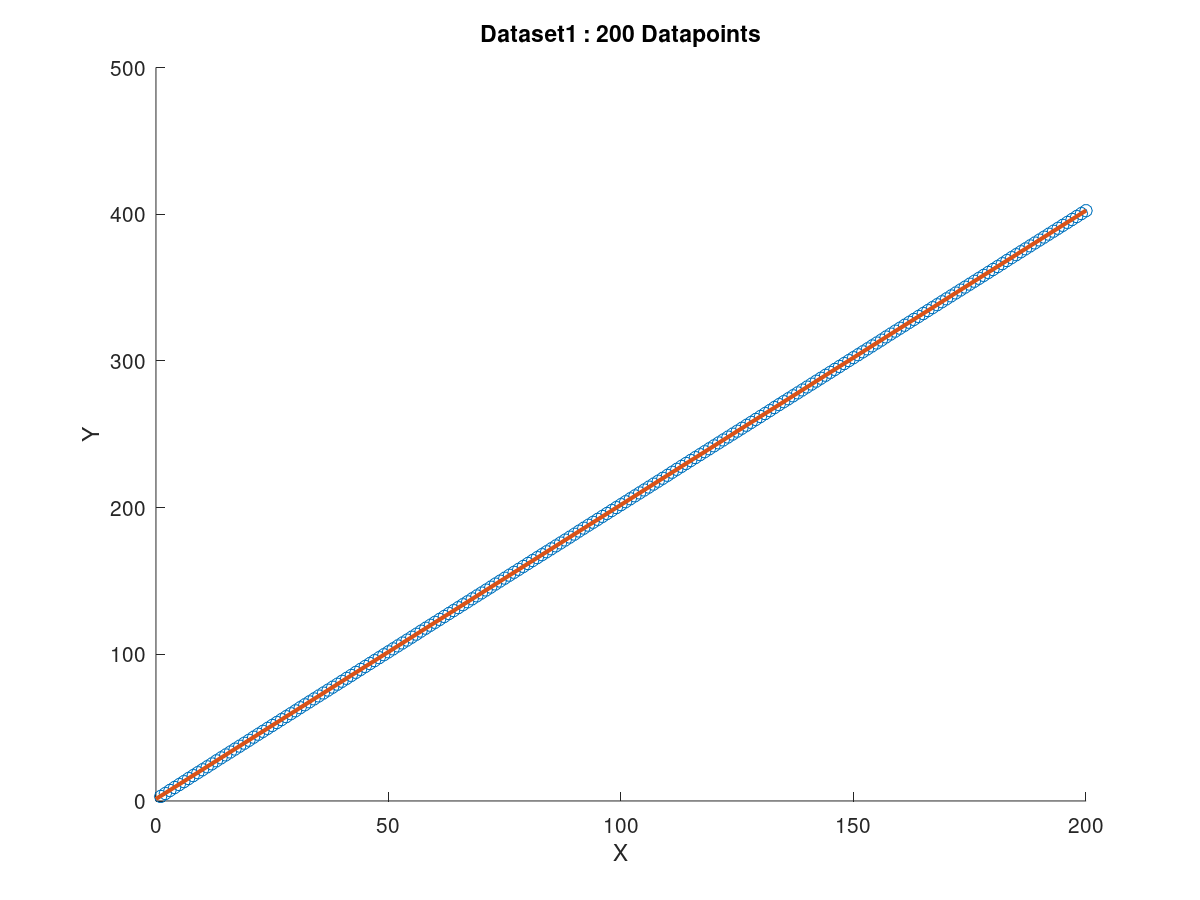
\includegraphics[width=1\textwidth]{D1-200.png}
	\label{fig:plots1}
\end{figure}
\pagebreak


\subsection{Dataset 2}
\begin{figure} [!ht]
	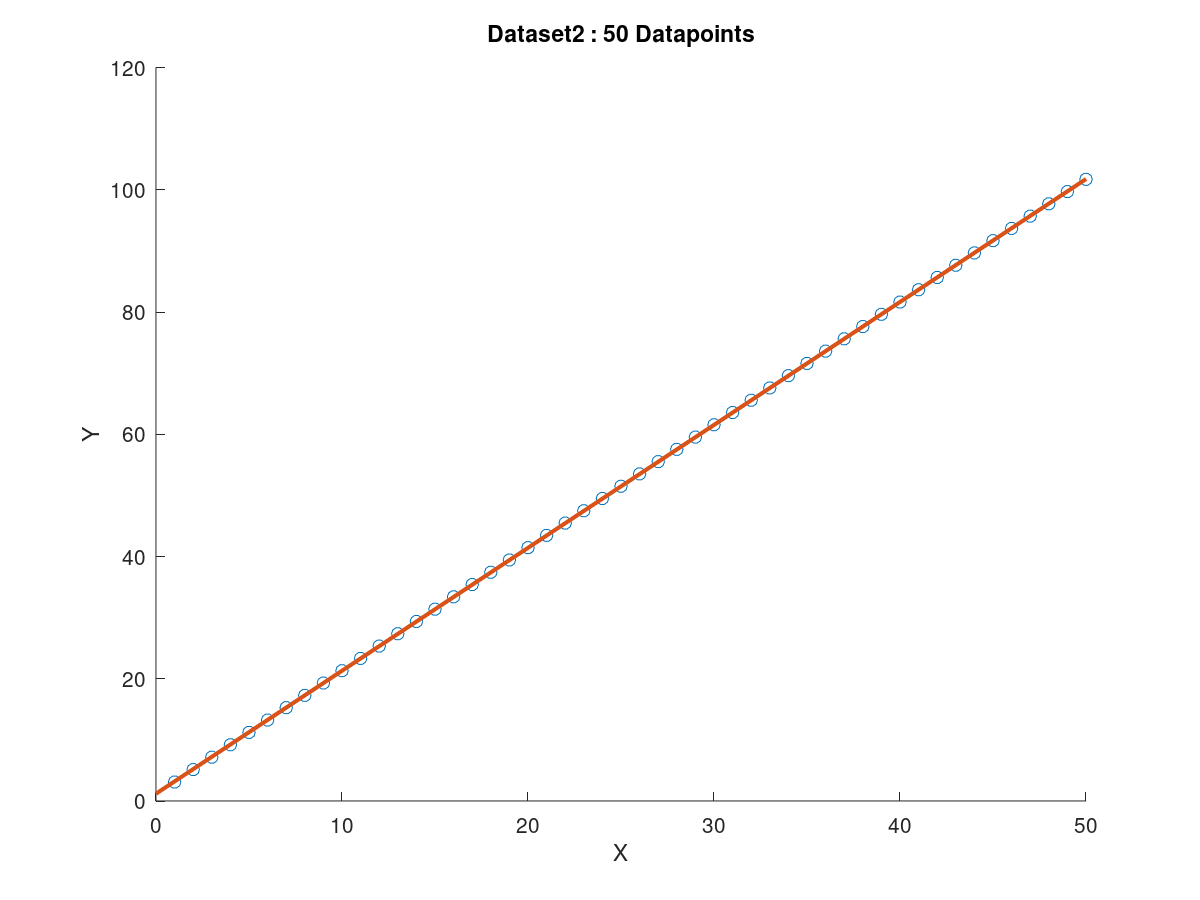
\includegraphics[width=.55\textwidth]{D2-50.png}\hfill
	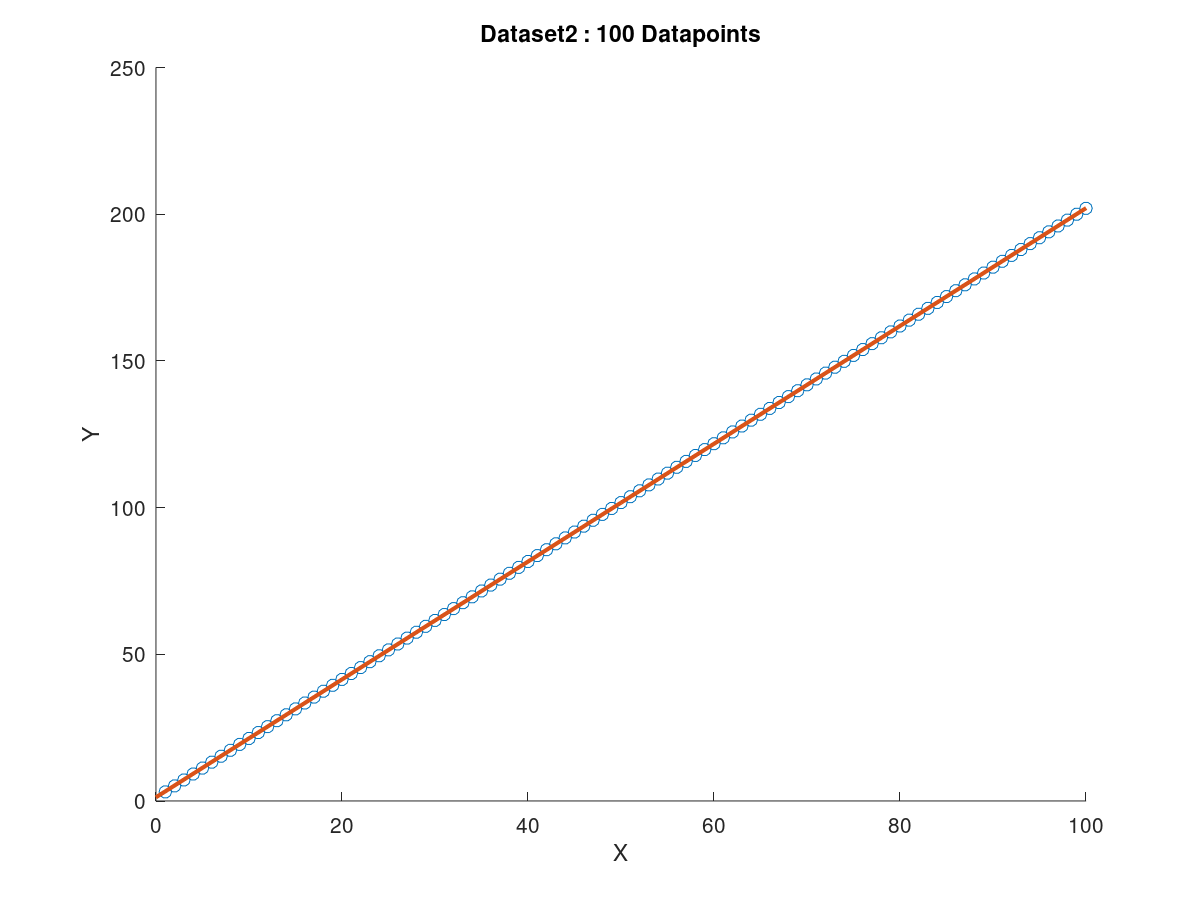
\includegraphics[width=.55\textwidth]{D2-100.png}\hfill
	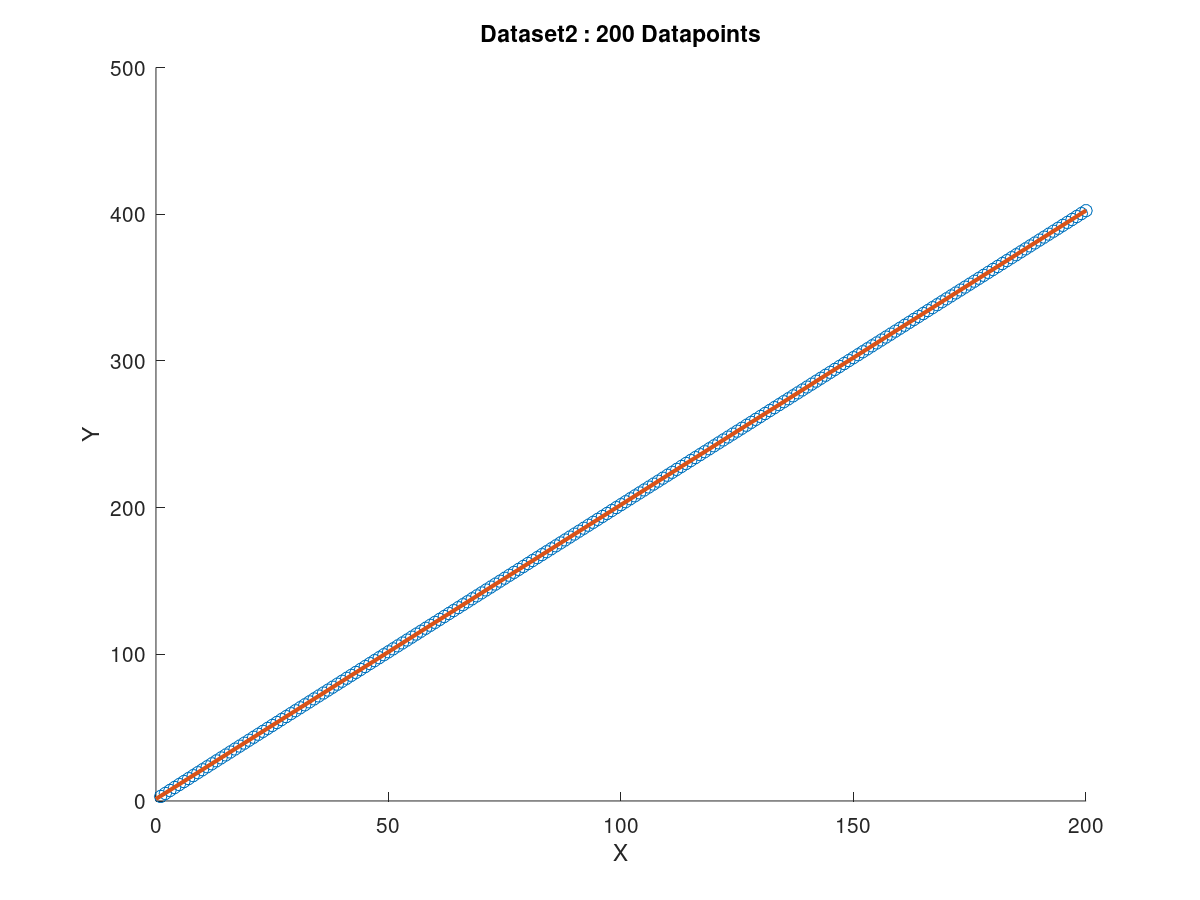
\includegraphics[width=1\textwidth]{D2-200.png}
	\label{fig:plots2}
\end{figure}
\pagebreak
\subsection{Dataset 3}
\begin{figure} [!ht]
	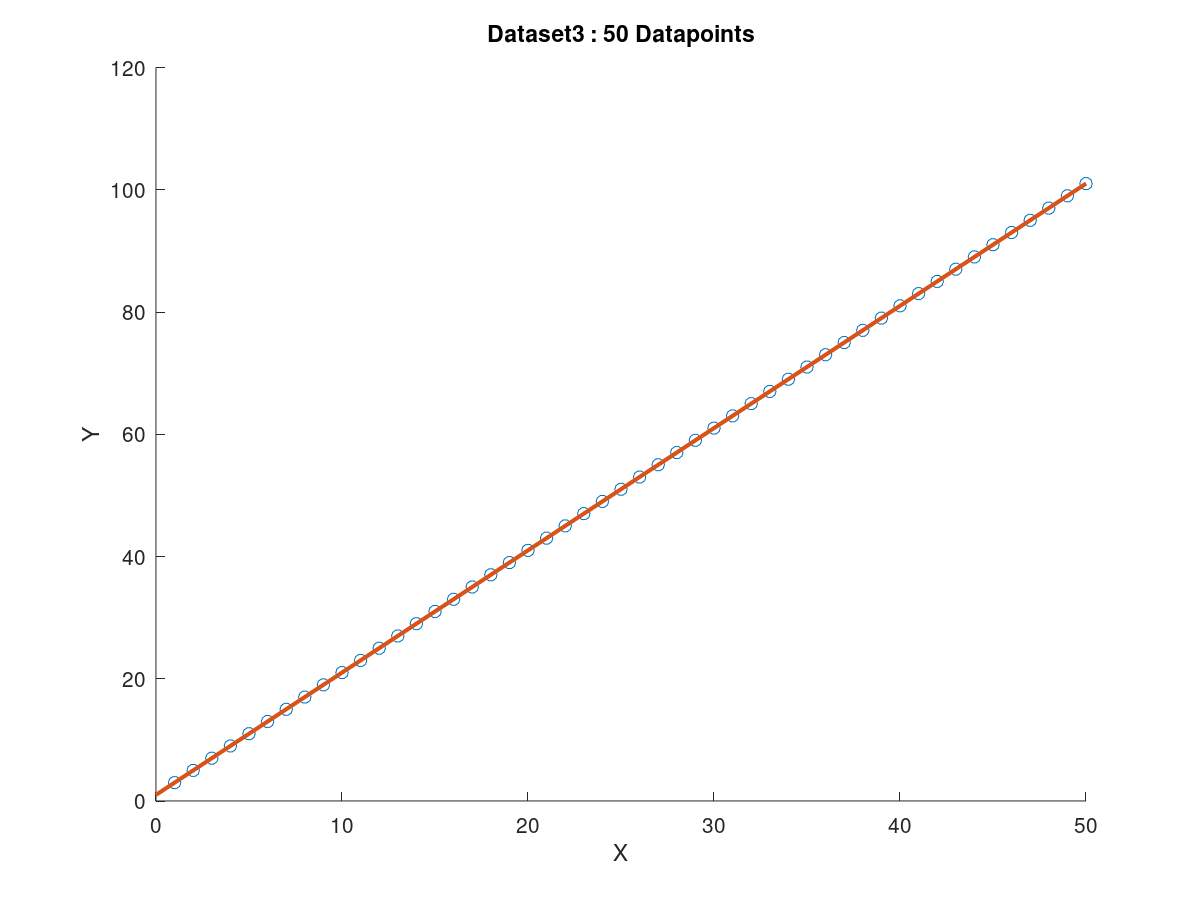
\includegraphics[width=.55\textwidth]{D3-50.png}\hfill
	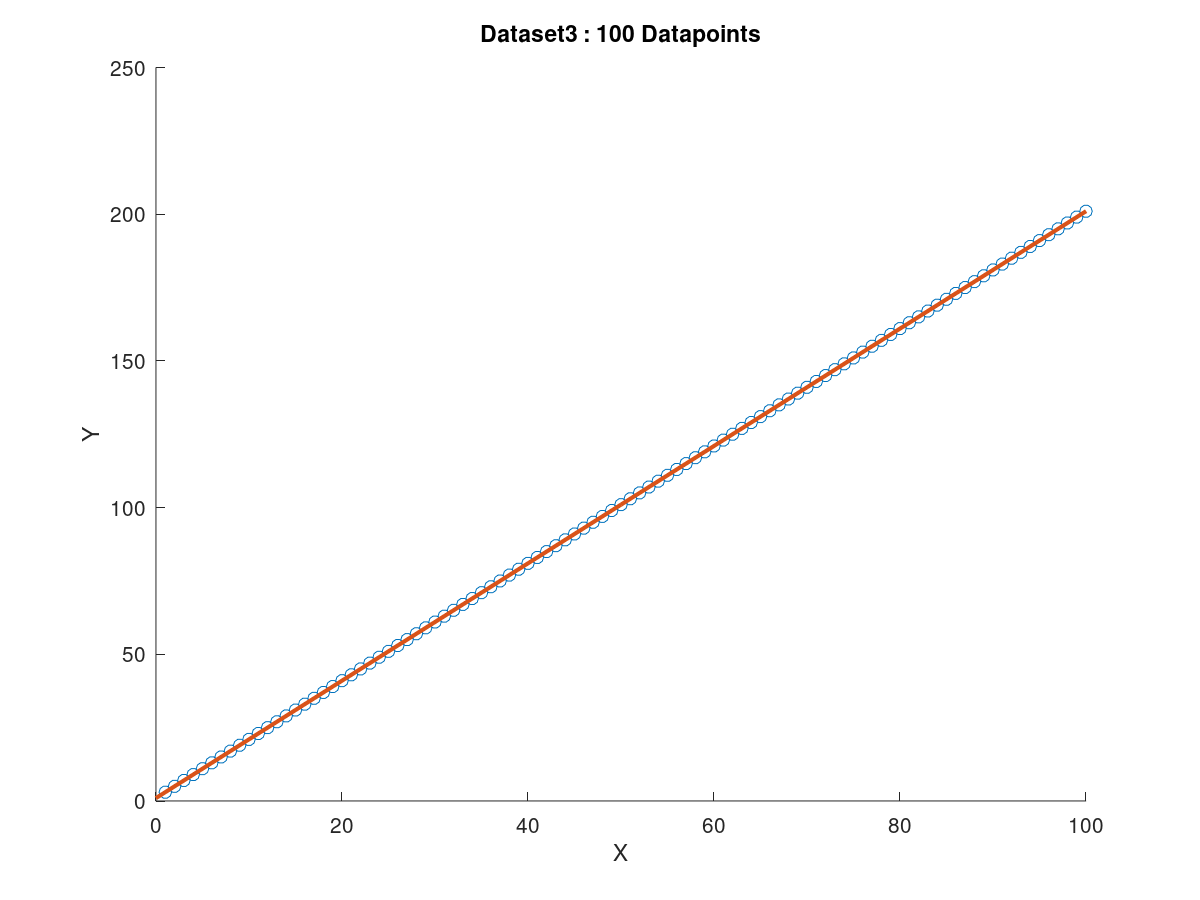
\includegraphics[width=.55\textwidth]{D3-100.png}\hfill
	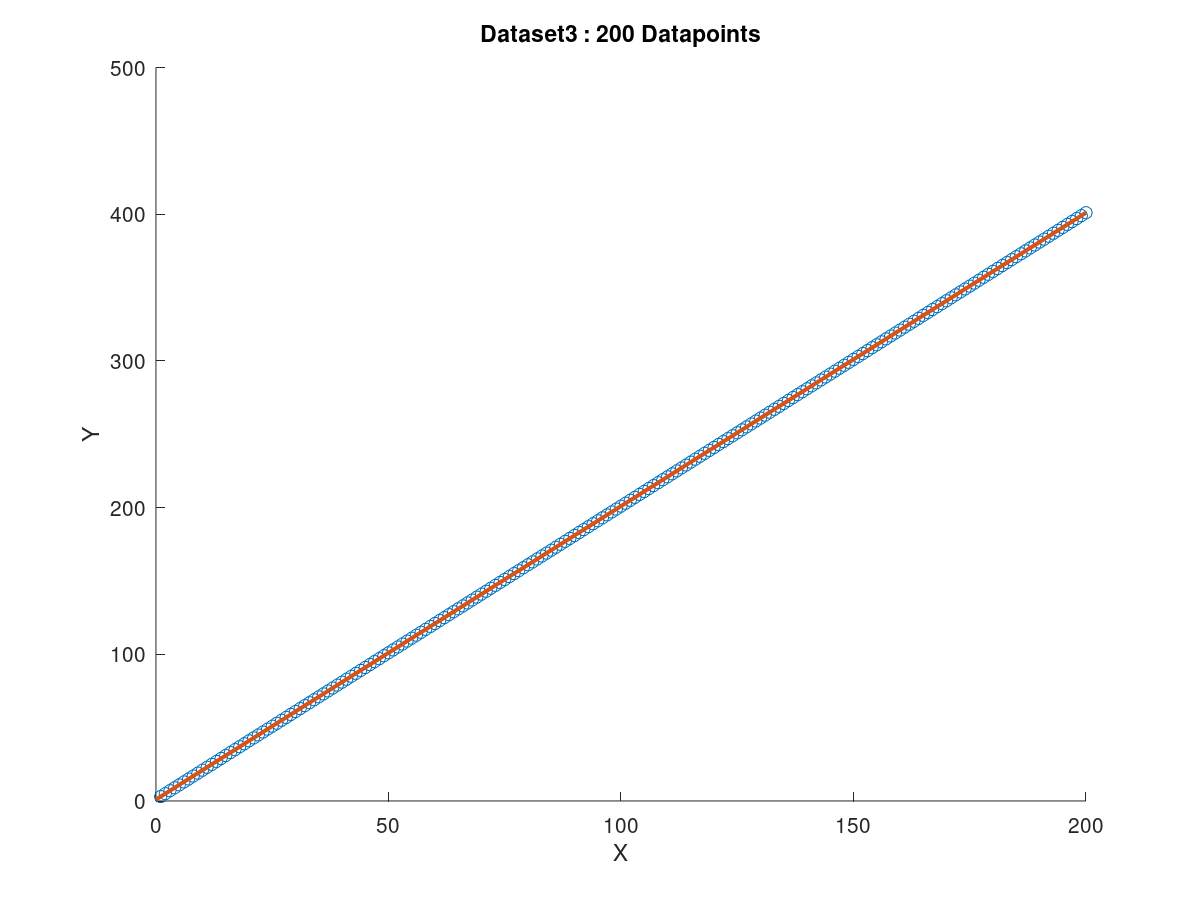
\includegraphics[width=1\textwidth]{D3-200.png}
	\label{fig:plots3}
\end{figure}
\end{document}